\documentclass[14pt,a4paper]{article}
\usepackage[utf8]{inputenc}
\usepackage{amsmath}
\usepackage{amsfonts}
\usepackage{amssymb}
\usepackage{tikz}
\usepackage{ifthen}
\usetikzlibrary{calc}
\usepackage{xcolor}
\usetikzlibrary{decorations.pathmorphing}
\usetikzlibrary{decorations.markings}

\colorlet{colP1}{gray!60}
\colorlet{colP2}{gray!20}
\colorlet{actcol}{blue!60}


\begin{document}

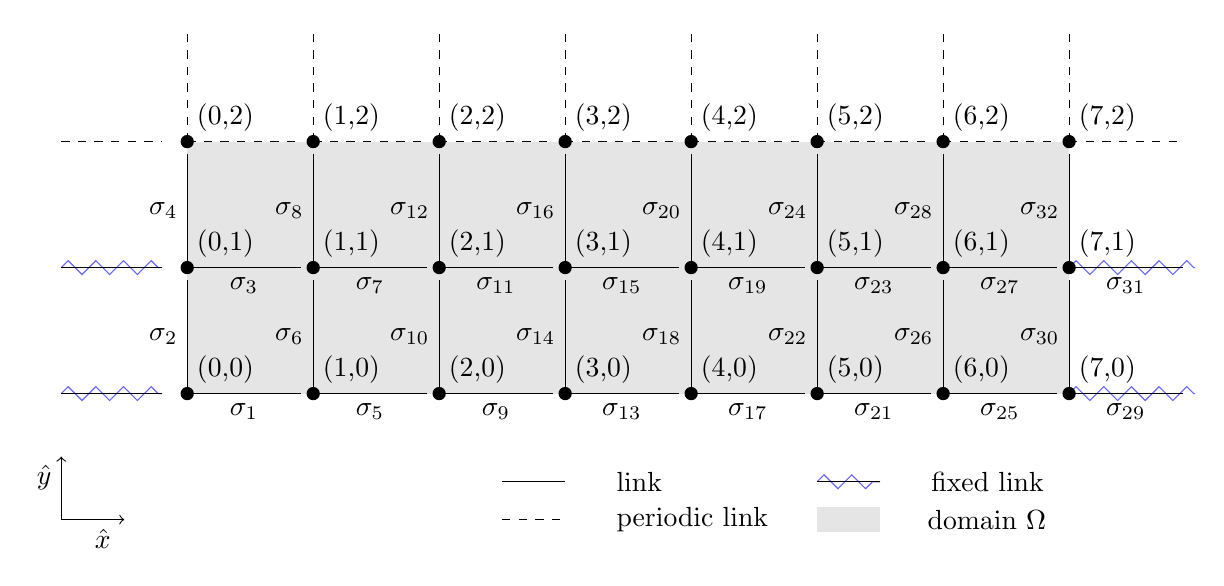
\begin{tikzpicture}[scale=1.6]
	
 % ================================================================  
 % Spatial
  % ================================================================  	
	\coordinate (A) at (0,0);
	\coordinate (B) at (7,2);
	\fill[colP2,thick] (A) rectangle (B);
	
	\coordinate (P1a) at (2.5,8.5);
	\coordinate (P1b) at (8.5,2.5);
	\coordinate (P2a) at (P1b);
	\coordinate (P2b) at (10,1);
	\coordinate (P3a) at (P1b);
	\coordinate (P3b) at (10,8.5);
	\coordinate (P4a) at (2.5,2.5);
	\coordinate (P4b) at (8.5,10);
	
	\coordinate (P5a) at (2.5,2.5);
	\coordinate (P5b) at (1,1);
	\coordinate (P6a) at (P1a);
	\coordinate (P6b) at (1,10);
	\coordinate (P4a) at (P3b);
	\coordinate (P4b) at (8.5,10);
	
	
	%\fill[dashed,colP1,thick] (P1a) rectangle (P1b);
	
	%\fill[dashed,colP1,thick] (P2a) rectangle (P2b);	
	
	%\fill[dashed,colP2,thick] (P3a) rectangle (P3b);	
	
	%\fill[dashed,colP1,thick] (P4a) rectangle (P4b);	
	
	%\fill[dashed,colP1,thick] (P5a) rectangle (P5b);	
	
	%\fill[dashed,colP1,thick] (P6a) rectangle (P6b);	

	 %% ----------------------------------------  
	 %%grid
	%\draw[step=2cm,black!60,thick] (0,0) grid (12,4);
	 % ----------------------------------------  
	 % boundary links
	  % ----------------------------------------  
        
        \draw[actcol, decorate, decoration=zigzag] (-1, 0) -- (-0.2,0) node [pos=0.66,below] {};
        \draw[-] (-1, 0) -- (-0.2,0) node [pos=0.66,below] {};
        \draw[actcol, decorate, decoration=zigzag] (-1, 1) -- (-0.2,1) node [pos=0.66,below] {};
        \draw[-] (-1, 1) -- (-0.2,1) node [pos=0.66,below] {};
        \draw[actcol, decorate, decoration=zigzag] (7, 1) -- (8,1) node [pos=0.66,below] {};
        \draw[actcol, decorate, decoration=zigzag] (7, 0) -- (8,0) node [pos=0.66,below] {};
        \draw[dashed] (-1, 2) -- (-0.2,2) node [pos=0.66,below] {};

        \newcounter{ga}\setcounter{ga}{0}
	\foreach \x in {0,1,...,7} 
	{	
		\foreach \y in {0,1,...,2} 
		{		
	        	  \ifthenelse{\x<8 \AND \y<2}
                         {
                          \stepcounter{ga}
                        \draw[-] (\x,\y ) -- (\x+0.9,\y) node [pos=0.5,below] {$\sigma_{\thega}$};
                          \stepcounter{ga}
                          \draw[-] (\x,\y ) -- (\x,\y+0.9) node [pos=0.5,left] {$\sigma_{\thega}$};
	         	}{
                            \draw[dashed] (\x,\y ) -- (\x,\y+0.9) node [pos=0.66,below] {};
                            \draw[dashed] (\x,\y ) -- (\x+0.9,\y) node [pos=0.66,below] {};
                          }
				
				
                          %\fill (\x+0.5,\y+0.5)  circle[radius=1.5pt] node [anchor=south west] {(\x,\y)};
                          \fill (\x,\y)  circle[radius=1.5pt] node [anchor=south west] {(\x,\y)};
					

				
		}	
	}	
	
	
	 % ----------------------------------------  
        \draw[->] (-1,-1 ) -- (-0.5,-1) node [pos=0.66,below] {$\hat{x}$};
      \draw[->] (-1, -1 ) -- (-1, -0.5) node [pos=0.66,left] {$\hat{y}$};
 
        %%%%%%%%%%%%%%%%%%%
        % Legend
        %%%%%%%%%%%%%%%%%%
        \draw[actcol, decorate, decoration=zigzag] (5,-0.7 ) -- (5.5,-0.7) node [pos=0.66,below] {};
        \draw[-] (5,-0.7 ) -- (5.5,-0.7) node [pos=1.66,right] {fixed link};
        \draw[-] (2.5,-0.7 ) -- (3,-0.7) node [pos=1.66,right] {link};
        \draw[dashed] (2.5,-1 ) -- (3,-1) node [pos=1.66,right] {periodic link};
        \fill[colP2,thick] (5,-0.9) rectangle (5.5,-1.1);
        \node [fill=white] at (5.8,-1) [right] {domain $\Omega$};
	 
	 
\end{tikzpicture}


\end{document}
